% Clast de documento
\documentclass[12pt, letterpaper]{article}

% Paquetes
\usepackage[utf8]{inputenc}
\usepackage[spanish]{babel}
\usepackage{biblatex}
\usepackage{csquotes}
\usepackage{graphicx}
\usepackage{datetime}
\usepackage{lipsum}
\usepackage{hyperref}
\usepackage{fancyhdr}
\usepackage{parskip}
\usepackage{amsmath}
\usepackage{listings}
\usepackage[table,xcdraw]{xcolor}
\usepackage{booktabs}
\usepackage{setspace}

%------------ 
% Decoración
%------------

% Configuración de colores de python
\lstset{
    language=Python,
    basicstyle=\ttfamily\small,
    keywordstyle=\color{blue},
    commentstyle=\color{green},
    stringstyle=\color{red},
    showstringspaces=false,
    numbers=left,
    numberstyle=\tiny\color{gray},
    frame=single,
    breaklines=true
}

\lstset{
    literate={á}{{\'a}}1 {é}{{\'e}}1 {í}{{\'\i}}1 {ó}{{\'o}}1 {ú}{{\'u}}1
             {Á}{{\'A}}1 {É}{{\'E}}1 {Í}{{\'I}}1 {Ó}{{\'O}}1 {Ú}{{\'U}}1
             {ñ}{{\~n}}1 {Ñ}{{\~N}}1
             {¡}{{!`}}1 {¿}{{?`}}1 % Añade caracteres especiales en español
}

% Configuración de header y footer
\pagestyle{fancy}
\fancyhf{}
\setlength{\headheight}{15.71667pt}
\addtolength{\topmargin}{-3.71667pt}

% Header
\fancyhead[L]{\textsc{\doctitle}}
\fancyhead[R]{\textit{\nouppercase{\rightmark}}}
\renewcommand{\sectionmark}[1]{%
  \markright{#1}%
}
\renewcommand{\subsectionmark}[1]{}

% Footer
\renewcommand{\footrulewidth}{0.4pt}
\fancyfoot[C]{Página \thepage}

% Título
\newcommand{\doctitle}{Modulación de señales}
\title{\doctitle}
\author{Juan Luis Serradilla Tormos}
\date{\monthname[\month] de \the\year}

% Bibliografía
\addbibresource{references.bib}
\ExecuteBibliographyOptions{sorting=none}


% Eliminar sangría
\setlength{\parindent}{0pt}

% Aumentar la separación entre párrafos
\setlength{\parskip}{1em plus 0.5em minus 0.2em}

% Doble espacio
\onehalfspacing{}


%-----------
% Documento
%-----------
\begin{document}

% Mostrar header y footer
\pagestyle{fancy}

% Mostrar el título
\maketitle

% Índice
\newpage
\tableofcontents

% Contenido
\newpage
\section{Introducción}
El Internet de las Cosas (IoT) consiste en una red de objetos físicos equipados con hardware y software que les permita conectarse e intercambiar datos a través de una red común~\cite{IoT-Oracle}. Al ser por tanto la comunicación entre dispositivos imprescindible en el IoT, las tecnologías de comunicación son un tema fundamental en este campo.

Este trabajo explorará las tecnologías de comunicación de los dispositivos IoT centrándose en la modulación de señales. Estas técnicas se utilizan para modificar las señales electromagnéticas para que puedan transmitir información. Por lo tanto, se investigarán sus fundamentos y funcionamiento, las tenoclogías y técnicas actuales, su implementación y los desafíos futuros.


\vspace{1em}
\section{Fundamentos de la Modulación de Señales}

La modulación de señales es un proceso fundamental en los sistemas de comunicación, ya que como se ha mencionado anteriormente la transmisión eficiente y onfiable de los datos es especialmente importante~\cite{modulacion-avsystem}.

En esencia, la modulación de señales consiste en modificar las propiedades de una onda portadora para transmitir información. 

\newpage
\begin{figure}[h]
    \centering
    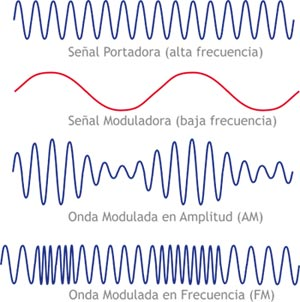
\includegraphics[width=6cm]{images/modulacion_ejemplo.jpg}
    \caption{Ejemplo de modulación de una onda portadora con una onda moduladora de baja frecuencia para transmitir información.}\label{fig:modulacion_ejemplo}
\end{figure}

Como se puede ver en la figura~\ref{fig:modulacion_ejemplo}, la modulación consta de una onda portadora y una onda moduladora, donde esta onda moduladora portará los datos digitales de los dispoisitvos IoT. Vamos a analizar más en detalle   estos dos roles.

\subsection{Frecuencia portadora}
Una señal portadora es una onda eléctrica que puede ser modificada en alguno de sus parámetros por la señal de información para obtener una señal modulada y que se transporta por el canal de comunicaciones~\cite{modulacion-radioacademy}.

Esta onda portadora también ayuda a solucionar el problema del tamaño de las antenas. El tamaño de una antena ($L$) debe ser proporcional a la longitud de la onda ($\lambda$), para así poder apreciar los cambios de la señal. Por ello, tenemos lo siguiente:
\begin{align}
    L \propto \lambda \propto \frac{1}{\nu}
\end{align}
donde $\nu$ es la frecuencia de la señal portadora. Esta característica hace que se puedan utilizar antenas de tamaño práctico para la transmisión inalámbrica.

Esta onda portadora también ayuda a que la señal enviada sea resistente al ruido.

\subsection{Frecuencia moduladora}
La onda moduladora es la onda que contiene la información digital que se quiere transmitir. Esta suele ser de una frecuencia más baja, por lo que necesita a la onda portadora para poder ser transmitida. El objetivo de esta onda es modificar algún parámetro de la onda portadora, como la amplitud, la frecuencia o la fase, para que la información pueda ser transmitida a través del canal de comunicación.

Las dos formas básicas de modulación son:
\begin{itemize}
    \item \textbf{Modulación de amplitud:} Este tipo de modulación consiste en variar el valor de la amplitud de la onda portadora en función de la onda moduladora. 

    \item \textbf{Modulación angular:} Este tipo de modulación consiste en variar el ángulo de la onda portadora. Para ello, se puede modificar tanto la frecuencia como la fase, pero manteniendo siempre la amplitud constante.
\end{itemize}

Otra forma de clasificar a la modulación es en función de cómo se realiza este proceso: de forma digital o de forma analógica. 

\begin{itemize}
    \item \textbf{Modulación analógica:} Este tipo de modulación realiza cambios continuos en la señal portadora, variando los parámetros de amplitud, frecuencia o fase de forma proporcional a la señal original. Podemos distinguir:
    \begin{itemize}
        \item Modulación AM
        \item Modulación FM
        \item Modulación PM
    \end{itemize}

    \item \textbf{Modulación digital:} En este tipo de modulación la señal moduladora es discreta (0 o 1). La información se codifica en símbolos (grupos de bits) que modifican la señal portadora de forma discontinua. Podemos distinguir:
    \begin{itemize}
        \item Modulación ASK
        \item Modulación FSK
        \item Modulación PSK
        \item Modulación QAM
    \end{itemize}
\end{itemize}

\subsection{Modulación digital sobre analógica}
A pesar de que existan dos tipos de modulación, en el contexto del IoT la modulación digital es la más utilizada. Esto se debe a varias razones:
\begin{itemize}
    \item \textbf{Sensibilidad al ruido:} La modulación analógica, especialmente AM, es más susceptible al ruido y las interferencias, lo que puede degradar la calidad de la señal transmitida. En entornos IoT donde los dispositivos pueden operar en condiciones ruidosas o con señales débiles, la robustez de la modulación digital ofrece una ventaja significativa.
    \item \textbf{Menor eficiencia espectral:} En general, las técnicas de modulación digital pueden ofrecer una mayor eficiencia espectral en comparación con las analógicas, lo que permite transmitir más datos dentro de un ancho de banda limitado. Esto es crucial en el espectro de radiofrecuencia cada vez más congestionado donde operan muchos dispositivos IoT.
    \item \textbf{Integración con sistemas digitales:} Dado que los dispositivos IoT operan con datos digitales, la modulación digital permite una integración más sencilla y directa con los circuitos y procesadores digitales. La conversión de señales analógicas a digitales y viceversa añade complejidad y puede introducir pérdidas.
    \item \textbf{Seguridad y cifrado:} Las técnicas de modulación digital se prestan mejor a la implementación de mecanismos de seguridad como el cifrado, que es cada vez más importante para proteger la confidencialidad e integridad de los datos transmitidos por los dispositivos IoT.
    \item \textbf{Eficiencia energética:} Muchas técnicas de modulación digital están diseñadas para ser energéticamente eficientes, lo cual es un requisito fundamental para los dispositivos IoT que funcionan con baterías y necesitan operar durante períodos prolongados.
\end{itemize}

\vspace{1em}
\section{Técnicas de modulación digital}
A continuación, se van a analizar las diferentes técnicas de modulación digital que se usan en el IoT.

\subsection{Modulación ASK y OOK}
La modulación ASK es un tipo de modulación de amplitud, por lo que los datos se representan variando la amplitud de la onda portadora. OOK por su parte es una forma de ASK donde la señal portadora se apaga y enciende para representar los bits 0 y 1~\cite{ask-unidad3}.

En ASK, la presencia de una onda portadora a una amplitud específica representa un bit 1, mientras que una amplitud diferente o la ausencia de la onda representa un bit 0. La fórmula para representar esta onda es la siguiente~\cite{modulacion-uv}:
\begin{align}
    U_{ASK}(t) = A \Big[1 \pm \frac{V(t)}{A} \Big] \cos(2\pi \nu_p t) = 
    A [1 \pm m(t)] \cos(2\pi \nu_p t) \label{eq:ask}
\end{align}

donde $V(t)$ es la señal moduladora, $A$ es la amplitud de la portadora, $\nu_p$ es la frecuencia de la portadora y $m(t)$ es la señal moduladora normalizada.

Se puede ver en la ecuación~\ref{eq:ask} que la amplitud de la señal portadora se modula en función de la seál portadora $V(t)$, pudiendo aumentar o disminuir dependiendo de cómo se haga la modulación.

\begin{figure}[h]
    \centering
    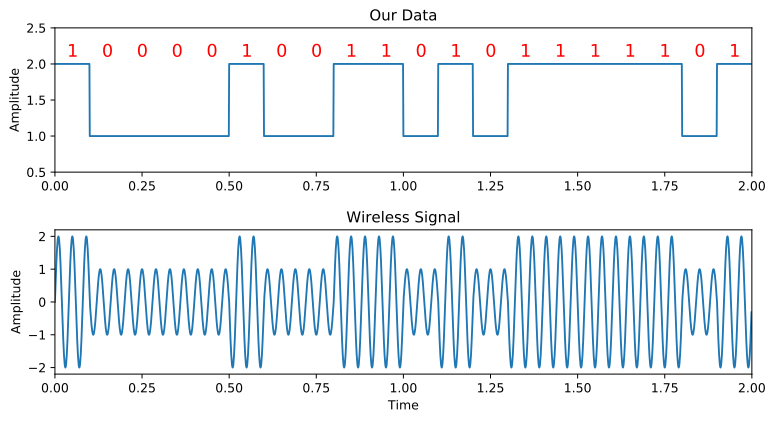
\includegraphics[width=9cm]{images/ASK.png}
    \caption{Ejemplo de modulación ASK.}\label{fig:ask}
\end{figure}

\newpage
Este tipo de modulación tiene sus ventajas y desventajas~\cite{ventajas-desventajas-ask}.
\begin{itemize}
    \item \textbf{Ventajas:}
    \begin{itemize}
        \item Es un método simple y fácil de implementar. Esto se debe a que, al solo tener que variar la amplitud moduladora para representar bits, solo hacen falta componentes simples como osciladores e interruptores. 
        \item Este método, en especial OOK, es muy eficiente  energéticamente. Esto se debe a que solo se transmite información cuando hay un ``1'', a diferencia de otros métodos que requieren la energía constante para mantener activa la portadora.
    \end{itemize}

    \item \textbf{Desventajas:}
    \begin{itemize}
        \item Es susceptible a las variaciones de amplitud y al ruido, debido a que es una transformación lineal. Es decir, si la amplitud de la señal portadora se ve afectada por el ruido, la señal modulada también se verá afectada de igual forma. Debido a esta distorsión los rangos de amplitud son limitados.
        \item Tiene menor eficiencia espectral que otros tipos de modulación. Esto se debe a varias razones; una de ellas es que transmite solo 1 bit por símbolo, en comparación con otros métodos como QAM que transmite 4 bits por símbolo. Esto a su vez hace que se necesiten más símbolos para enviar la misma cantidad de información, lo que amplia el ancho de banda necesario.
    \end{itemize}
\end{itemize}

\subsection{Modulación FSK}
La modulación FSK (Frequency Shift Keying) es un tipo de modulación digital que utiliza dos o más frecuencias diferentes para representar los bits 0 y 1. En este caso, la frecuencia de la señal portadora se cambia en función de la señal moduladora.

Podemos definir la señal FSK con la siguiente expresión~\cite{modulacion-uv}:
\begin{align}
    U_{FSK}(t) =
    \left\{
    \begin{array}{l}
        A \cos(2\pi\nu_1 t + \theta_p) \quad 
        \text{si } \nu_1 = \nu_p + \Delta\nu_p \Leftrightarrow \text{``1''} \\
        A \cos(2\pi\nu_2 t + \theta_p) \quad
        \text{si } \nu_2 = \nu_p - \Delta\nu_p \Leftrightarrow \text{``0''}
    \end{array}
    \right. \label{eq:fsk}
\end{align}

Podemos ver en la ecuación~\ref{eq:fsk} cómo esta vez la amplitud $A$ permanece constante, y simplemente tenemos dos ecuaciones de ondas diferentes dependiendo de la frecuencia que se esté utilizando. Cuando la frecuencia moduladora es $\nu_1 > \nu_p$, se representa un bit 1, y cuando es $\nu_2 < \nu_p$ se representa un bit 0. Podemos ver un ejemplo de modulación FSK en la figura~\ref{fig:fsk}.
\begin{figure}[h]
    \centering
    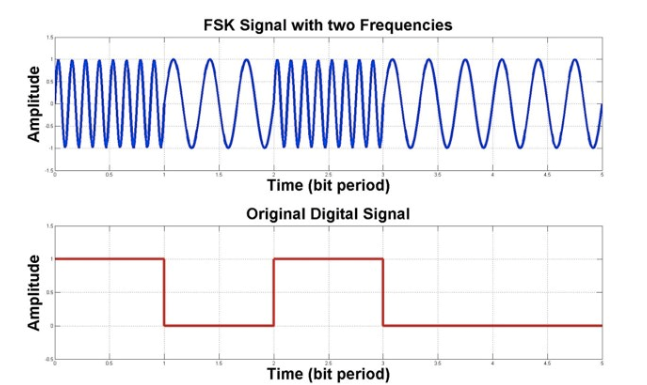
\includegraphics[width=9cm]{images/FSK.png}
\caption{Ejemplo de modulación FSK.\label{fig:fsk}}
\end{figure}

Este tipo de modulación tiene sus ventajas y sus desventaja~\cite{ask-unidad3}.
\begin{itemize}
    \item \textbf{Ventajas:}
    \begin{itemize}
        \item Tiene una buena resistencia al ruido y a la interferencia. Esto se debe a que la información se transmite a través de cambios en la frecuencia, lo que hace que sea menos susceptible a las variaciones de amplitud y a las interferencias externas.
        \item Las modulaciones FSK tienen una envolvente de amplitud constante, lo que reduce la necesidad de amplificadores lineales en el transmisor y permite una amplificación de potencia más eficiente.
        \item Los transmisores y receptores FSK son fáciles de implementar para aplicaciones de baja velocidad de datos.
    \end{itemize}

    \item \textbf{Desventajas:}
    \begin{itemize}
        \item Las ténicas FSK, al igual que ASK, necesitan más ancho de banda que las técnicas PSK y QAM para la misma velocidad de datos. 
        \item La velocidad de datos alcanzada suele ser menor que la que se consigue con técnicas más modernas y complejas.
        \item La técnica FSK es sensible al desplazamiento de frecuencia en los osciladores transmisor y el receptor, lo que puede degradar el rendimiento.
    \end{itemize}
\end{itemize}

\subsection{Modulación PSK, QPSK y Modulación de Orden Superior}
La modulación PSK (Phase Shift Keying) es un tipo de modulación digital en la cuál se modifica la fase de la señal portadora para representar la información. En su forma más sencilla, BPSK (Binary Phase Shift Keying), se utilizan dos fases diferentes (0ºy 180º) para representar los bits 0 y 1~\cite{modulacion-uv}:
\begin{align}
    U_{PSK}(t) =
    \left\{
    \begin{array}{l}
        A \cos(2\pi\nu_p t) \Leftrightarrow \text{``1''} \\
        A \cos(2\pi\nu_p t + \pi) \Leftrightarrow \text{``0''}
    \end{array}
    \right.
\end{align}

Se puede ver un ejemplo de modulación PSK en la figura~\ref{fig:psk}.
\begin{figure}[h]
    \centering
    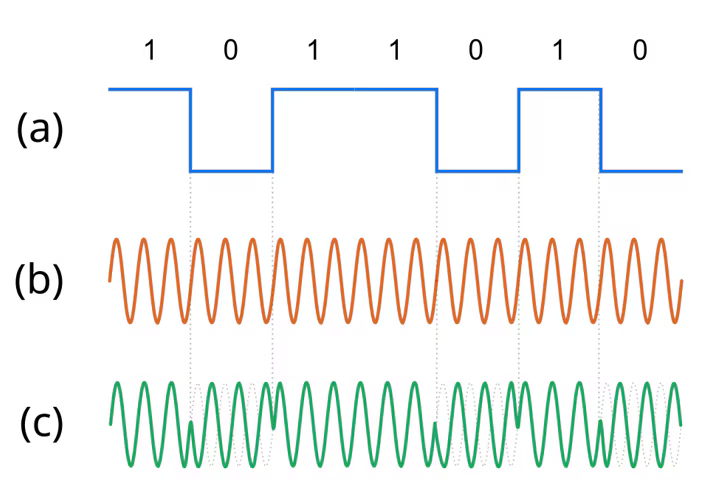
\includegraphics[width=9cm]{images/PSK.png}
    \caption{Ejemplo de modulación PSK.\label{fig:psk}}
\end{figure}

Otro tipo de modulación PSK es la modulación por desplazamiento de fase en cuadratura (QPSK), que utiliza cuatro fases diferentes (0º, 90º, 180º y 270º) para representar dos bits de información a la vez. Esto permite una mayor eficiencia espectral en comparación con BPSK.\@

La modulación PSK tiene sus ventajas y desventajas~\cite{inproceedings}.
\begin{itemize}
    \item \textbf{Ventajas:}
    \begin{itemize}
        \item La modulación PSK ofrece una mayor eficiencia espectral en comparación con ASK y FSK, transmitiendo más datos en un menor ancho de banda. Esto se nota sobretodo en QPSK y modulaciones de mayor orden, como 8PSK o 16PSK.\@
        \item Tiene una buena resistencia al ruido en comparación con ASK, ya que la información se codifica en la fase, que es menos susceptible que la amplitud.
        \item Al igual que FSK, tiene una envolvente de amplitud constante, lo que permite el uso de amplificadores de potencia no lineales más eficientes.
    \end{itemize}

    \item \textbf{Desventajas:}
    \begin{itemize}
        \item Los moduladores y demoduladores PSK son más complejos que los ASK y FSK a la hora de implementarlos, especialmente los de orden superior.
        \item La modulación PSK suele necesitar una demodulación coherente para un rendimiento óptimo, lo que requiere circuitos de recuperación de portadora más complejos en el receptor.
        \item Cuanto mayor es el orden de la modulación, a pesar de que se transmite más información la resistencia al ruido en la fase disminuye, provocando errores si la fase de referencia no es estable.
    \end{itemize}
\end{itemize}

\subsection{Modulación OFDM}
La técnica OFDM no es una modulación como tal, sino una forma de combinar varias modulaciones para transmitir más información. Esta técnica de modulación digital divide el ancho de banda disponible en múltiples subportadoras ortogonales, transmitiendo datos en paralelo en estas subportadoras. Las ondas ortogonales son señales cuyos valles y picos no se suporponen, cumpliendo así la siguiente condición:
\begin{align}
    \int_{0}^{T} \Phi_1(t) \Phi_2(t) dt = 0
\end{align}

donde $\Phi_1(t)$ y $\Phi_2(t)$ son las ondas ortogonales y $T$ es el periodo de la señal. Cada subportadora se modula mediante un esquema de modulación de baja velocidad de datos, como QAM o PSK.\@ Las subportadoras están espaciadas de manera precisa para garantizar la ortogonalidad, lo que evita la interferencia entre ellas.

Vamos a desglosar el funcionamiento de OFDM.\@ Como se ha mencionado, lo primero que se hace es generar $N$ subportadoras. Luego, la suma de las $N$ subportadoras crea un símbolo OFDM ($U_{OFDM}$). También se añade un prefijo cíclico ($CP$) y un espacio temporal entre los símbolos para evitar la interferencia entre símbolos (ISI). 

El proceso de envío es el siguinete:
\begin{enumerate}
    \item Se agrupan los bits en símbolos.
    \item Cada símbolo se asigna a una subportadora.
    \item Se convierten las subportadoras en al dominio del tiempo desde el dominio de la frecuencia mediante la Transformada Inversa de Fourier (IFFT).
    \item Se añade el CP al símbolo OFDM.\@
    \item Se envía la señal.
\end{enumerate}

En el caso de querer recibir la señal, el proceso es el siguiente:
\begin{enumerate}
    \item Se elimina el prefijo cíclico (CP).
    \item Se transforma la señal del dominio del tiempo al dominio de la frecuencia mediante la Transformada de Fourier (FFT).
    \item Se demodulan las subportadoras para obtener los símbolos.
    \item Se convierten los símbolos en bits.
\end{enumerate}

\newpage
Podemos ver un esquema de la modulación OFDM en la figura~\ref{fig:ofdm}.
\begin{figure}[h]
    \centering
    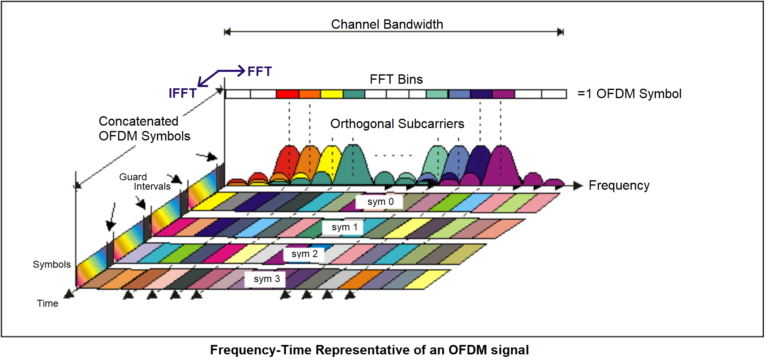
\includegraphics[width=9cm]{images/OFDM.png}
    \caption{Esquema de la modulación OFDM.\label{fig:ofdm}}
\end{figure}

Esta técnica de modulación tiene varias ventajas y desventajas.
\begin{itemize}
    \item \textbf{Ventajas:}
    \begin{itemize}
        \item La modualción OFDM ofrece una muy alta eficiencia espectral al transmitir múltiples subportadoras juntas dentro de un ancho de banda dado.
        \item Esta modulación es altamente resistente desvanecimiento selectivo en frecuencia y a la interferencia multitrayecto, ya que cada subportadora experimenta un desvanecimiento plano.
        \item La ecualización en el receptor es más sencilla, ya que cada subportadora puede ser tratada de forma independiente.
    \end{itemize}

    \item \textbf{Desventajas:}
    \begin{itemize}
        \item Las señales OFDM pueden tener una alta relación potencia pico a promedio, lo que requiere amplificadores lineales de alta calidad para evitar la distorsión.
        \item La señal OFDM es sensible a los desplazamientos en frecuencia y a la deriva.
        \item Los sistemas OFDM requieren el uso de la Transformada Rápida de Fourier (FFT) y la Transformada Rápida de Fourier Inversa (IFFT), lo que aumenta la complejidad de la implementación.
    \end{itemize}
\end{itemize}

\subsection{Modulación de Espectro Ensanchado CSS}

La Modulación de Espectro Ensanchado (Spread Spectrum Modulation) es una técnica de comunicación inalámbrica en la que la señal transmitida se distribuye intencionalmente sobre un ancho de banda mucho mayor que el mínimo necesario para enviar la información.

Algunos ejemplos de modulación de espectro ensanchado son la modulación por salto de frecuencia (FHSS), la modulación por secuencia directa (DSSS) y la modulación de espectro ensanchado por código de secuencia (CSS).\@ Esta última es utilizada por el protocolo LoRaWAN.\@

Para entender cómo funciona la modulación CSS es necesario comprender primero qué es un chirp. Un chirp es una señal cuya frecuencia cambia de forma continua a lo largo del tiempo. El funcionamiento de la modulación CSS es el siguiente:
\begin{enumerate}
    \item Se agrupan los bits en símbolos.
    \item Se crea un chirp de referencia que barre todo el ancho de bada $B$ en un tiempo $T$. Por ejemplo, si $B = 125 kHz$ y $T = 1 ms$, el chirp barrerá 125 kHz/ms.
    \item Cada símbolo se representa mediante un desplazamiento crítico en el chirp base. Por ejemplo, si el símbolo es $3$ el chirp transmitido comienza en $f_{\min} + 3\Delta f$. Finalmente el receptor compara el chirp con el chirp base para decodificar el símbolo.
\end{enumerate}

\newpage
Podemos ver un ejemplo de modulación CSS en la figura~\ref{fig:css}.
\begin{figure}[h]
    \centering
    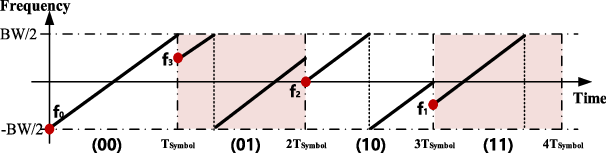
\includegraphics[width=11cm]{images/CSS.png}
    \caption{Ejemplo de chirps resultantes en una modulación CSS.\label{fig:css}}
\end{figure}

Esta técnica de modulación tiene varias ventajas y desventajas.
\begin{itemize}
    \item \textbf{Ventajas:}
    \begin{itemize}
        \item La modulación CSS es altamente resistente al ruido y a la interferencia, lo que la hace ideal para aplicaciones de IoT en entornos ruidosos.
        \item Esta técnica permite una alta eficiencia energética, lo que es crucial para dispositivos IoT alimentados por batería.
        \item La modulación CSS permite la coexistencia de múltiples dispositivos en el mismo canal de comunicación sin interferencias significativas.
    \end{itemize}

    \item \textbf{Desventajas:}
    \begin{itemize}
        \item CSS ofrece una excelente sensibilidad del receptor, lo que permite la comunicación a largas distancias con bajos niveles de potencia.
        \item La dispersión de la señal sobre un ancho de banda amplio hace que CSS sea muy resistente a las interferencias de banda estrecha y al ruido.
        \item La naturaleza de espectro ensanchado de CSS proporciona resistencia al desvanecimiento multitrayecto y al efecto Doppler.
    \end{itemize}

    \item \textbf{Desventajas:}
    \begin{itemize}
        \item La velocidad de datos alcanzable con CSS suele ser menor en comparación con las técnicas de modulación de banda estrecha debido a la dispersión de la señal en un ancho de banda mayor.
        \item El procesamiento de señales de chirp puede ser más complejo que el de esquemas de modulación más simples.
    \end{itemize}
\end{itemize}

\vspace{1em}
\section{Implementación y aplicación en IoT}
La implementación de técnicas de modulación en IoT se adapta a los requisitos específicos de cada aplicación, buscando un equilibrio entre el consumo de energía, el alcance, la velocidad de datos y la resistencia a las interferencias.

Vamos a ver algunos ejemplos prácticos de qué modulación usar en cada caso.
\begin{itemize}
    \item En hogares inteligentes, Zigbee, con O-QPSK o BPSK, facilita redes de baja potencia para dispositivos como luces y sensores, priorizando el bajo consumo y la capacidad de malla.
    \item Las cámaras de seguridad inteligentes emplean Wi-Fi con OFDM y QAM (un tipo de modulación AM) para la transmisión de video de alta resolución, requiriendo altas velocidades de datos.
    \item En la agricultura inteligente, LoRaWAN con modulación CSS permite la comunicación de largo alcance y bajo consumo para sensores que monitorizan las condiciones del suelo y el clima en grandes extensiones.
    \item Para el seguimiento de activos y la lectura inteligente de contadores, NB-IoT utiliza principalmente $\pi/2$-BPSK y QPSK, ofreciendo buena cobertura y bajo consumo a través de redes celulares.
    \item En la automatización industrial, donde la fiabilidad y la baja latencia son cruciales, se están explorando tecnologías como 5G con modulación QAM de orden superior y OFDM para soportar la comunicación en tiempo real y el control de maquinaria.
    \item Los sistemas de identificación por radiofrecuencia (RFID) a menudo utilizan la modulación ASK o PSK para la comunicación de corto alcance y bajo consumo de energía~\cite{yin2025low}. En aplicaciones de telemetría médica, se utiliza ASK debido a su bajo consumo de energía y simplicidad. Los controles remotos para puertas de garaje y sistemas de entrada sin llave también emplean ASK.\@
    \item La modulación FSK se encuentra en sistemas de buscapersonas para mensajes de texto, redes de sensores inalámbricos de baja potencia, y en Bluetooth y BLE a través de GFSK.En el ámbito del hogar inteligente, los termostatos y sistemas de seguridad inalámbricos pueden utilizar FSK para una comunicación robusta.
    \item QPSK es ampliamente utilizado en sistemas de comunicación por satélite, redes inalámbricas y comunicaciones por fibra óptica.En el contexto del IoT, se investiga su uso en sistemas de retrodispersión ambiental. También es la modulación empleada en IEEE 802.11b y NB-IoT.
    \item OFDM es la base de Wi-Fi para dispositivos IoT que requieren altas velocidades de datos.También se está considerando para NB-IoT para mejorar la eficiencia y la capacidad~\cite{cardarilli2021design}.
\end{itemize}


\vspace{1em}
\section{Conclusiones}
La modulación de señales es un componente fundamental de las comunicaciones de dispositivos IoT, ya que permite la transmisión eficiente y fiable de datos entre una amplia gama de dispositivos y aplicaciones. La elección de la técnica de modulación adecuada depende de una compleja interacción de factores, incluyendo los requisitos de la aplicación en términos de alcance, velocidad de datos, consumo de energía y robustez frente a las interferencias, así como las limitaciones de costo y complejidad de los dispositivos IoT.

Las técnicas de modulación digital como ASK y OOK son simples y de bajo consumo, ideales para aplicaciones de bajo ancho de banda y corto alcance como RFID y controles remotos. FSK ofrece una mayor robustez al ruido, lo que la hace adecuada para aplicaciones como redes de sensores inalámbricos y Bluetooth. PSK y QPSK proporcionan una mejor eficiencia espectral y robustez, encontrando uso en tecnologías como NB-IoT y algunos protocolos de corto alcance. Las técnicas avanzadas como OFDM son esenciales para aplicaciones de alta velocidad de datos como Wi-Fi, mientras que el espectro ensanchado por chirp (CSS) en LoRaWAN destaca en comunicaciones de bajo consumo y largo alcance.

\printbibliography[title={Bibliografía}]
\addcontentsline{toc}{section}{Referencias}
\end{document}
